\section{L10-Conduzione}
Per \textbf{conduzione termica} si intende la trasmissione di calore per contatto molecolare diretto. Il principio alla base della conduzione è diverso a seconda della struttura fisica del corpo: se la conduzione termica avviene nei gas è dovuta alla diffusione atomica e molecolare, se invece avviene nei liquidi e nei solidi è a causa di onde elastiche; nei materiali metallici il fenomeno è principalmente dovuto alla diffusione degli elettroni liberi dato che è trascurabile il contributo dell’oscillazione elastica del reticolo cristallino.
\subsection{Strumeti matematici}
\subsubsection{Operatore nabla}
\[
    \vec{\nabla} = \frac{\delta}{\delta x} \vec{i} + \frac{\delta}{\delta y} \vec{j} + \frac{\delta}{\delta z} \vec{k}
\]
\[
    \vec{\nabla} T = grad(T) = \frac{\delta T}{\delta x} \vec{i} + \frac{\delta T}{\delta y} \vec{j} + \frac{\delta T}{\delta z} \vec{k}
\]
\[
    \vec{\nabla} \cdot  \vec{v} = div(\vec{v}) = \frac{\delta \vec{v}_x}{\delta x} \vec{i} + \frac{\delta \vec{v}_y}{\delta y} \vec{j} + \frac{\delta \vec{v}_z}{\delta z} \vec{k}
\]
\[
    \vec{\nabla} \cdot  \vec{\nabla} T = \nabla^2 T = \;\text{laplaciano di}\;T = \frac{\delta^2 T}{\delta x^2} \vec{i} + \frac{\delta^2 T}{\delta y^2} \vec{j} + \frac{\delta^2 T}{\delta z^2} \vec{k}
\]
\subsubsection{Teorema della divergenza (o di Gauss)}
\[
    \oint_S \vec{v} \cdot \vec{n} dS = \int_{V} div(\vec{v}) dV
\]
\subsection{Equazione generale della conduzione}
Il postulato di Fourier è uno strumento incompleto ai fini della soluzione di un
problema di conduzione. Da esso però si può dedurre un'equazione
fenomenologica denominata equazione di Fourier o equazione generale della
conduzione, la cui soluzione consente di determinare la distribuzione di
temperatura in un mezzo. Questa equazione esprime il bilancio di energia di un
sistema sede di trasmissione del calore per conduzione:
\begin{center}
    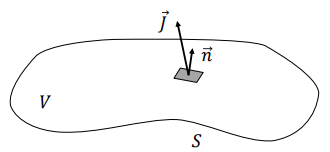
\includegraphics[height=4cm]{../L10/img2.PNG}
\end{center}
Bilancio di energia:
\[
    \frac{\delta U}{\delta t} = \dot{Q}^\leftarrow + \dot{\Sigma}
\]
dove $\frac{\delta U}{\delta t}$ è la variazione di energia nel tempo che può essere espressa in maniera più generale come $\frac{\delta}{\delta t} \int_{V} \rho u d V$ (fino ad ora nel corso abbiamo considerato situazioni in cui tutto era omogeneamente distribuito, qui però stiamo considerando casi in cui nello spazio una proprietà può variare. Con questo integrale si ottiene il valore medio), $\dot{Q}^\leftarrow$ è la potenza entrante e $\dot{\Sigma}$ è la sorgente di potenza.
\[
    \frac{\delta}{\delta t} \int_{V} \rho u d V = - \oint_S \vec{j} \cdot  \vec{n} dS + \int_{V} \sigma dV
\]
Applichiamo ora il teorema della divergenza:
\[
    \frac{\delta}{\delta t} \int_{V} \rho u dV = - \int_{V} div(\vec{j}) dV + \int_{V} \sigma dV
\]
Con le ipotesi di colume $V$ e densità $\rho$ indipendenti dal tempo si ottiene:
\[
    \int_{V} \rho \frac{\delta u}{\delta t} dV + \int_{V} div(\vec{j}) dV - \int_{V} \sigma dV = 0
\]
\[
    \int_{V}\left[\rho \frac{\delta u}{\delta t} + div(\vec{j}) - \sigma)\right]dV
\]
Per cui si ha valido per qualunque volume:
\[
    \rho \frac{\delta u}{\delta t} + div(\vec{j}) - \sigma = 0
\]
La variazione di energia interna è esprimibile attraverso la relazione $du = c_v dT$ e sfruttando inoltre il postulato di Fourier $\vec{j} = - k grad (T)$ si ottiene
\[
    \rho c_v \frac{\delta T}{\delta t} = div (k \cdot grad(T)) + \sigma
\]
con l'ipotesi di materiale omogeneo ed isotropo ($k$ costante) si ottiene l'\textbf{equazione generale della conduzione o equazione di Fourier}
\[
    \rho c_v \frac{\delta T}{\delta t} = k \nabla^2T + \sigma
\]
Questa equazione viene anche scritta come 
\[
    \frac{1}{a} \frac{\delta T}{\delta t} = \nabla^2 T + \frac{\sigma}{k}
\]
con $a = \frac{k}{\rho c_v}$ la \textbf{diffusività termica} in $[m^2/s]$.
\newline
\newline
L'equazione di Fourier è una equazione differenziale alle derivate parziali e 
\begin{itemize}
    \item lineare in $T= f(x,y,z,t)$;
    \item sel secondo ordine rispetto a $x,y,z$;
    \item del primo ordine rispetto a $t$.
\end{itemize}
\subsection{Condizioni al contorno}
L’equazione di Fourier non è risolvibile in assenza di ulteriori informazioni, quali
\begin{itemize}
    \item \textbf{condizione iniziale} (se il problema è tempo invariante, noi ci limiteremo a casi stazionari);
    \item \textbf{condizioni al contorno} (o ai limiti)
\end{itemize}
\ \newline
La soluzione richiede quindi che sia \textbf{noto}:
\begin{itemize}
    \item la geometria del mezzo in cui abbiene la conduzione (simmetrie, dimensioni indefinite, etc);
    \item le proprietà delle sorgenti termiche (massa volumica $rho$, calore specifico $c_V$, conduttività termica $k$, in molti casi li consideremo costanti per semplificare gli esercizi);
    \item le distribuzioni delle sorgenti termiche (tendenzialmente diremo che sarà uniformemente distribuita e costante nel tempo);
    \item la distribuzione della temperatura nel mezzo all'istante iniziale (se si è nel caso tempo invariante);
    \item le condizioni al contorno superficiale relative all'interazione tra il mezzo e ciò che lo delimita.
\end{itemize}
\ \newline
Per quanto riguarda le condizioni al contorno, vale la seguente \textbf{terminologia}:
\begin{itemize}
    \item \textbf{Problema di Dirichlet} (condizione di primo tipo): quando è assegnata la distribuzione della funzione $T$ (temperatura) in ogni punto del contorno, eventualmente in funzione del tempo
    \[
        T = T(\vec{x},t) \;\;\;\;\;\;\;\;\;\;\vec{x} \in S
    \]
    Il problema di Dirichlet è un problema in cui si va a impostare la temperatura.
    \item \textbf{Problema di Neumann} (condizione di secondo tipo): quando è assegnata al contorno la derivata normale della funzione $T$, eventualmente in funzione del tempo
    \[
        \frac{\delta T}{\delta \vec{n}} = f(\vec{x},t) \;\;\;\;\;\;\;\;\;\; \vec{x} \in S
    \]
    Questa condizione rappresenta, in senso fisico, la conoscenza del \textbf{flusso termico areico} alla superficie del sistema.\newline
    \newline
    In questo caso, invece di assegnare direttamente la grandezza, andiamo ad assegnare la derivata della grandezza, in particolare assegnamo un grandiente della temperatura, che è strettamente legato al flusso termico.
    \item \textbf{Problema di Cauchy} (condizione di terzo tipo): quando è assegnata al contorno una combinazione lineare della funzione $T$ e della sua derivata normale, eventualmente in funzione del tempo
    \[
        \frac{\delta T}{\delta \vec{n}} + A T = f(\vec{x}, t) \;\;\;\;\;\;\;\;\;\; \vec{x} \in S; \;\; A = \text{costante}\;
    \]
    Questa condizione si verifica nella maggior parte dei casi quando vi è scambio termico per convezione alla superficie di controllo del sistema. Si ottiene, avendo indicato con $h$ il coefficiente convettivo:
    \[
        -k \frac{\delta T}{\delta \vec{n}} = h (T-T_{\infty}) \;\;\;\;\;\;\;\;\;\; \vec{x} \in S
    \]
    essendo $T_{\infty}$ la temperatura di un eventuale fluido esterno (e non dipende da $T$, è una costante).\newline
    \newline
    Il problema di Cauchy è un po' un mix dei problemi di primo e di secondo tipo: vengono combinati il gradiente della temperatura e la temperatura stessa.
    \item \textbf{Condizione di quarto tipo}: questa condizione corrisponde al caso in cui si ha scambio termico attraverso l'interfaccia di due mezzi in cui è presente un trasporto conduttivo ed aventi diversa conduttività termica ($k_1$ e $k_2$)
    \[
        -k_1 \frac{\delta T_1}{\delta \vec{n}} = -k_2 \frac{\delta T_2}{\delta \vec{n}} \;\;\;\;\;\;\;\;\;\; \vec{x} \in S
    \]
    in cui $T_1$ e $T_2$ sono le funzioni che descrivono il campo di temperatura nei mezzi rispettivamente di conduttività $k_1$ e $k_2$.\newline
    \newline
    In questo caso siamo in presenza di due mezzi, ciascuno con il proprio flusso termico individuato dall'assengazione del proprio gradiente.\newline
    \newline
    Se il contatto tra i due mezzi materiali è perfetto, può allora essere specificata una ulteriore relazione tra le temperature superficiali dei mezzi:
    \[
        T_1 = T_2 \;\;\;\;\;\;\;\;\;\; \vec{x} \in S
    \]
    Nel caso reale invece c'è sempre un salto termico fra i due mezzi, ma per semplificare la trattazione considereremo le temperature identiche.
\end{itemize}
\subsection{Sistema di coordinate}
Nell’impostare il problema differenziale è inoltre importante scegliere
opportunamente il sistema di coordinate nel quale esplicitare l’operatore di
Laplace.
\begin{itemize}
    \item Coordinate cartesiane ortogonali $T = T(x,y,z)$:
    \[
        \nabla^2T = \frac{\delta^2T}{\delta x^2} + \frac{\delta^2T}{\delta y^2} + \frac{\delta^2T}{\delta z^2}
    \]
    \item Coordinate cilindriche $T = T(r, \theta, z)$:
    \[
        \nabla ^2 T = \frac{1}{r} \frac{\delta }{\delta r} \left(r \frac{\delta T}{\delta r}\right) + \frac{1}{r^2}\frac{\delta^2 T}{\delta \theta^2} + \frac{\delta^2 T}{\delta z^2}
    \]
    \item Coordinate sferiche $T = T(r, \theta, \psi)$:
    \[
        \nabla^2 T = \frac{1}{r^2} \frac{\delta}{\delta r}\left(r^2 \frac{\delta T}{\delta r}\right) + \frac{1}{r^2 sin^2(\psi)}\frac{\delta^2 T}{\delta \theta^2} + \frac{1}{r^2 sin(\psi)}\frac{\delta}{\delta\psi}\left(sin(\psi)\frac{\delta T}{\delta \psi}\right)
    \]
\end{itemize}
\subsection{Conduzione 1D con generazione interna}
L’equazione generale di Fourier in regime stazionario, con generazione interna
(costante), monodimensionale diventa:
\begin{itemize}
    \item In coordiante cartesiane ortogonali $T = T(x)$:
    \[
        \frac{d^2T}{dx^2} + \frac{\sigma}{k} = 0
    \]
    \item In coordiante cilindriche $T= T(r)$:
    \[
        \frac{1}{r} \frac{d}{dr}\left(r \frac{dT}{dr}\right) + \frac{\sigma}{k} = 0
    \]
    \item In coordinate sferiche $T =T(r)$:
    \[
        \frac{1}{r^2} \frac{d}{dr}\left(r^2 \frac{dT}{dr}\right) + \frac{\sigma}{k} = 0
    \]
\end{itemize}
Integrando diventa:
\begin{itemize}
    \item In coordiante cartesiane ortogonali $T = T(x)$:
    \[
        T = -\frac{\sigma}{2k} x^2 + Ax + B
    \]
    \item In coordiante cilindriche $T= T(r)$:
    \[
        T = - \frac{\sigma}{4k}r^2 + C ln(r) + D
    \]
    \item In coordinate sferiche $T =T(r)$:
    \[
        T = - \frac{\sigma}{6k}r^2 + \frac{E}{r} + F
    \]
\end{itemize}
Le \textbf{costanti di integrazione} ($A,B,C,D,E,F$) sono determinabili con le \textbf{condizioni al contorno}.
\subsection{Parete piana indefinita}
Si consideri il caso senza generazione interna $T = Ax + B$. \newline
\newline
Si consideri il caso di \textbf{due condizioni di prima specie}:
\begin{center}
    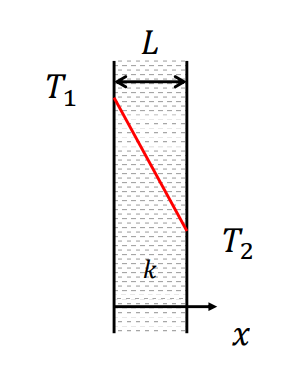
\includegraphics[height=4cm]{../L10/img1.PNG}
\end{center}

\[
    \begin{cases}
        x = 0\\ T = T_1
    \end{cases} \;\;\;\;\;\;\;\;\;\;\;\;\;\;\; \begin{cases}
        x = L\\ T = T_2
    \end{cases} \;\;\;\;\;\;\;\;\;\;\;\;\;\;\; \begin{cases}
        T_1 = B \\ T_2 = AL+B
    \end{cases}
\]
\[
    T = T_1 - \frac{T_1-T_2}{L}x
\]
\[
    J = - k \frac{dT}{dx} \;\;\;\;\;\;\;\;\;\;\;\;\;\;\; J = k \frac{T_1-T_2}{L} = \text{costante}
\]
$J =$ costante è intuibile dal bilancio energetico che afferma che la potenza netta entrante in un volume di controllo deve essere nulla (non si accumula energia).\newline
\newline
Il flusso termico complessivo è dato per una superficie $S$:
\[
    \dot{Q} = k S \frac{T_1-T_2}{L}
\]
\[
    \dot{Q} = \frac{T_1-T_2}{R_{cond}}
\]
dove $R_{cond}$ è la \textbf{resistenza termica di tipo conduttiva} e vale $R_{cond} = \frac{L}{kS}$.\newline
\newline
Analogia elettrica $\Delta V = RI$.\newline
\newline
Caso di una \textbf{Parete composta}:
\begin{center}
    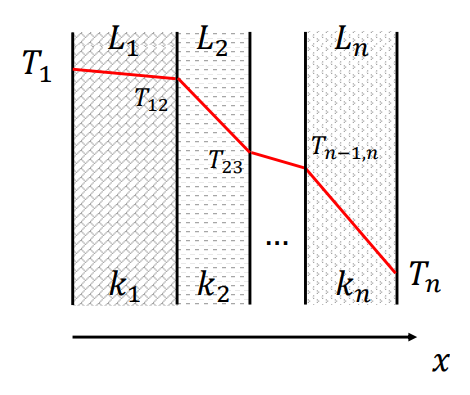
\includegraphics[height=4cm]{../L10/img3.PNG}
\end{center}
\[
    \begin{matrix}
        \dot{Q} = \frac{T_1-T_{12}}{R_1}\\
        \dot{Q} = \frac{T_{12} - T_{23}}{R_2}\\
        \dots\\
        \dot{Q} = \frac{T_{n-1,n} - T_{n}}{R_n}
    \end{matrix}  
\]
\[
    \dot{Q} = \frac{T_1-T_n}{R_{eq}}
\]
Resistenze in serie
\[
    R_{eq} = \sum_{i=1}^{n}R_i
\]
Il gradiente di temperatura (pendenza) nella parete è inversamente proporzionale alla conduttività termica del mezzo.\newline
\newline
Caso di condizioni al contorno di \textbf{terza specie (tipo convettivo)} $T= Ax + B$
\begin{center}
    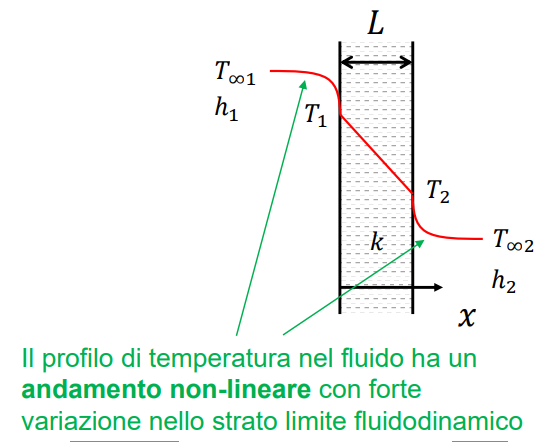
\includegraphics[height=5cm]{../L10/img4.PNG}
\end{center}
\[
    \begin{cases}
        x = 0 \\ h_1(T_{\infty 1}-T) = -k \frac{dT}{dx}
    \end{cases} \;\;\;\;\;\;\;\;\;\;\;\;\;\;\; \begin{cases}
        x = L\\ -k \frac{dT}{dx} = h_2(T-T_{\infty 2})
    \end{cases}
\]
\[
    \begin{cases}
        h_1(T_{\infty 1} - B) = -k A \\ -kA = h_2 (AL+B - T_{\infty 2})
    \end{cases}
\]
\[
    A = - \frac{(T_{\infty 1} - T_{\infty 2})}{\left(\frac{1}{h_1} + \frac{L}{k} + \frac{1}{h_2}\right)} \frac{1}{k}
\]
\[
    B = -\frac{(T_{\infty 1} - T_{\infty 2})}{\left(\frac{1}{h_1} + \frac{L}{k} + \frac{1}{h_2}\right)} \frac{1}{h_1} + T_{\infty 1}
\]
\[
    T = - \frac{(T_{\infty 1} - T_{\infty 2})}{\left(\frac{1}{h_1} + \frac{L}{k} + \frac{1}{h_2}\right)}\left(\frac{x}{k} + \frac{1}{h_1}\right) + T_{\infty 1}
\]
\ \newline
\newline
Caso di condizioni al contorno di \textbf{terza specie (tipo convettivo)} $T = Ax + B$
\begin{center}
    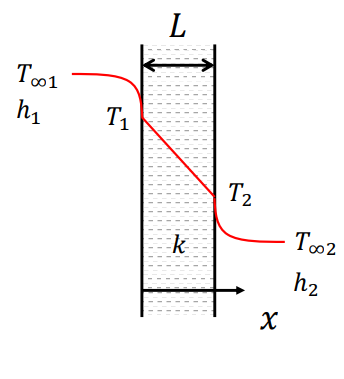
\includegraphics[height=4cm]{../L10/img5.PNG}
\end{center}

\[
    \dot{Q} = \frac{T_{\infty 1}- T_{1}}{\frac{1}{h_1 S}} \;\;\;\;\;\;\;\;\;\; \dot{Q} = \frac{T_1-T_2}{\frac{L}{kS}} \;\;\;\;\;\;\;\;\;\;\;\;\;\;\; \dot{Q} = \frac{T_2-T_{\infty 2}}{\frac{1}{h_2S}}
\]
\[
    \dot{Q} = \frac{T_{\infty 1} - T_{\infty 2}}{\frac{1}{S}\left(\frac{1}{h_1} + \frac{L}{k} + \frac{1}{h_2}\right)} \;\;\;\;\;\;\;\;\;\;\;\;\;\;\; \dot{Q} = \frac{T_{\infty 1} - T_{\infty 2}}{R_{eq}}
\]
\[
    R_{eq} = \frac{1}{S}\left(\frac{1}{h_1} + \frac{L}{k} + \frac{1}{h_2}\right)
\]
Con \textbf{resistenza termica di tipo convettiva} $R_{conv} = \frac{1}{hS}$.
\subsection{Barra cilindrica piena (con generazione di potenza)}
Caso di condizioni al contorno di \textbf{prima specie}
\begin{center}
    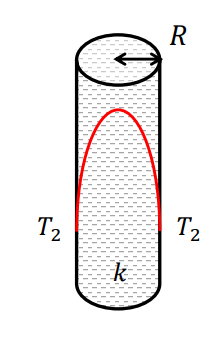
\includegraphics[height=4cm]{../L10/img6.PNG}
\end{center}

\[
    T= - \frac{\sigma}{4k} r^2 + C ln(r) + D \;\;\;\;\;\;\;\;\;\; \frac{dT}{dr} = - \frac{\sigma}{2k}r + \frac{C}{r}
\]
\[
    \begin{cases}
        r = 0 \\ \frac{dT}{dr} = 0
    \end{cases} \;\;\;\;\;\;\;\;\;\;\;\;\;\;\;  \begin{cases}
        r=R \\ T=T_2 
    \end{cases}\;\;\;\;\;\;\;\;\;\;\;\;\;\;\; \begin{cases}
        C=0 \\ D = T_2 + \frac{\sigma}{4k} R^2
    \end{cases}
\]
\[
    T = \frac{\sigma}{4k} (R^2 - r^2) + T_2 \;\;\;\;\;\;\;\;\;\;\;\;\;\;\; \frac{dT}{dr}  = - \frac{\sigma}{2k}r
\]
\[
    J = -k \frac{dT}{dr} = \frac{\sigma}{2} r \;\;\;\;\;\;\;\;\;\;\;\;\;\;\; \frac{\dot{Q}}{L} = \frac{JA}{L} = \pi r^2 \sigma
\]
con $A$ l'area dello scambio temrico
\subsection{Cilindro cavo (senza generazione di potenza)}
Caso di condizioni al contorno di \textbf{prima specie}
\begin{center}
    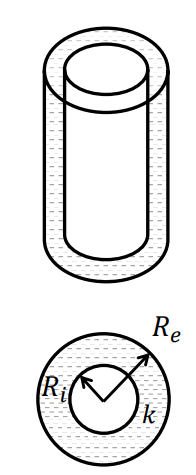
\includegraphics[height=3cm]{../L10/img7.PNG}
\end{center}
\[
    T= C ln(r) + D
\]
\[
    \begin{cases}
        r = R_i \\ T = T_i
    \end{cases} \;\;\;\;\;\;\;\;\;\;\;\;\;\;\;\begin{cases}
        r= R_e \\ T=T_e 
    \end{cases}\;\;\;\;\;\;\;\;\;\;\;\;\;\;\; \begin{cases}
        T_i = C ln(R_i) + D \\ T_2 = C ln (R_e) + D
    \end{cases}
\]
\[
    T_e-T_i = C(ln(R_e) - ln(R_i))
\]
\[
    T= \frac{T_e-T_i}{ln\left(\frac{R_e}{R_i}\right)}ln(r) + T_i - \frac{T_e-T_i}{ln\left(\frac{R_e}{R_i}\right)}ln(R_i) = T_i + \frac{T_e-T_i}{ln\left(\frac{R_e}{R_i}\right)}ln\left(\frac{r}{R_i}\right)
\]
\[
    J = -k \frac{dT}{dr} = k \frac{T_i-T_e}{ln\left(\frac{R_e}{R_i}\right)} \frac{1}{r}
\]
\[
    \frac{\dot{Q}}{L} = \frac{JA}{L} = \frac{(T_i-T_e)}{\frac{1}{2\pi k}ln\left(\frac{R_e}{R_i}\right)}
\]
\[
    \dot{Q} = \frac{(T_i-T_e)}{\frac{1}{2\pi L k}ln\left(\frac{R_e}{R_i}\right)} \;\;\;\;\;\;\;\;\;\;\;\;\;\;\; \dot{Q} = \frac{(T-i-T_e)}{R_{cond}}
\]
con $R_{cond} = \frac{1}{2 \pi L k}ln\left(\frac{R_e}{R_i}\right)$ \textbf{resistenza termica di tipo conduttiva}.\newline
\newline
Si ha un andamento logaritmico della temperatura nella parete solida:
\begin{center}
    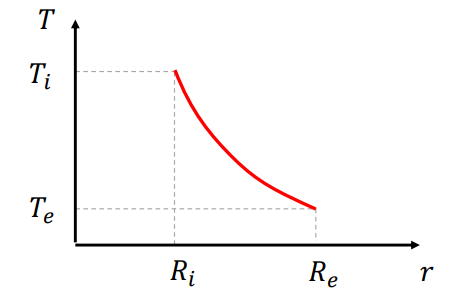
\includegraphics[height=3cm]{../L10/img8.PNG}
\end{center}
\ \newline
\newline
Caso di condizioni al contorno di \textbf{terza specie (tipo convettivo)}
\[
    \dot{Q} = \frac{(T_{\infty i}-T_{\infty 2})}{\frac{1}{2\pi L}\left( \frac{1}{h_i R_i} + \frac{1}{k}ln\left(\frac{R_e}{R_i}\right) + \frac{1}{h_eR_e}\right)}
\] 
\[
    \dot{Q}= \frac{(T_{\infty i} - T_{\infty e})}{R_{eq}}
\]
\textbf{Resistenza termica di tipo convettiva}: $R_{conv} = \frac{1}{2\pi L h R}$
\newline
\newline
\textbf{Raggio critico di isolamento}:
\[
    \dot{Q} = \frac{(T_i - T_e)}{R_{eq}}
\]
con $T_i$ temperatura fluido interno e $T_e$ temperatura fluido esterno.
\begin{center}
    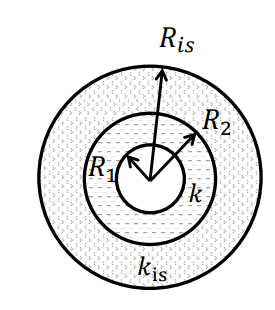
\includegraphics[height=3cm]{../L10/img9.PNG}
\end{center}
\[
    R_{eq} = \frac{1}{2\pi L}\left( \frac{1}{h_i R_1} + \frac{1}{k} ln \left(\frac{R_2}{R_1}\right) + \frac{1}{K_{is}} ln \left(\frac{R_{is}}{R_2}\right) + \frac{1}{h_eR_{is}}\right)
\]
\begin{center}
    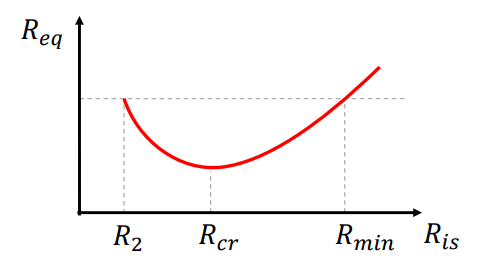
\includegraphics[height=3cm]{../L10/img10.PNG}
\end{center}
\[
    \frac{dR_{eq}}{dR_{is}} = \frac{1}{2 \pi L} \left(\frac{1}{k_{is} R_{is}} - \frac{1}{h_e R_{is}^2}\right)
\]
\[
    \rightarrow R_{cr} = \frac{k_{is}}{h_e}
\]
\subsection{Parete sferica cava (senza generazione di potenza)}
caso di condizioni al contonro di \textbf{prima specie}
\begin{center}
    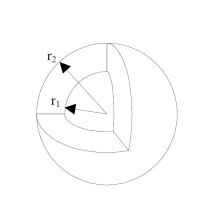
\includegraphics[height=3cm]{../L10/img11.PNG}
\end{center}
\[
    T = \frac{E}{r} + F \;\;\;\;\;\;\;\;\;\;\;\;\;\;\;\frac{dT}{dr} = - \frac{E}{r^2}
\]
\[
    \begin{cases}
        r = R_1 \\ T= T_1
    \end{cases} \;\;\;\;\;\;\;\;\;\;\;\;\;\;\;\begin{cases}
        r=R_2 \\ T=T_2
    \end{cases} \;\;\;\;\;\;\;\;\;\;\;\;\;\;\; \begin{cases}
        T_1 = \frac{E}{R_1} + F \\ T_2 = \frac{E}{R_2}+ F
    \end{cases}
\]
\[
    T= T_1 + (T_1-T_2) \frac{\frac{1}{r} - \frac{1}{R_1}}{\frac{1}{R_1} - \frac{1}{R_2}}
\]
\[
    \dot{Q} = \frac{T_1-T_2}{\frac{1}{4 \pi k} \left( \frac{1}{R_1}- \frac{1}{R_2} \right)}
\]
\[
    \dot{Q}= \frac{(T_1-T_2)}{R_{cond}}
\]
\[
    J = k \frac{T_1-T_2}{\frac{1}{R_1}- \frac{1}{R_2}} \frac{1}{r^2}
\]
\textbf{resistenza termica di tipo conduttiva}: $R_{cond} = \frac{1}{4\pi k} \left( \frac{1}{R_1} - \frac{1}{R_2} \right)$
\subsection{Conduttività termica}
Valori indicativi per diversi materiali in condizioni normali di temperatura e pressione
\begin{center}
    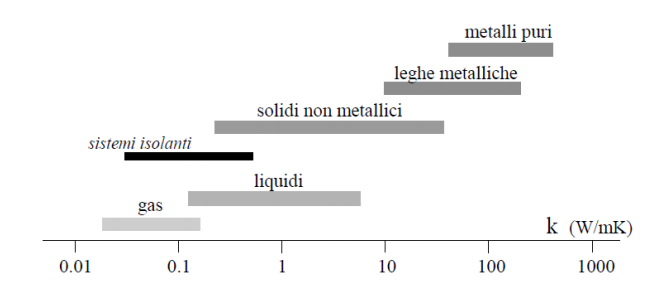
\includegraphics[height=3cm]{../L10/img12.PNG}
\end{center}
\ \newline
Valori indicativi per diversi materiali in condizioni normali di temperatura e pressione
\begin{center}
    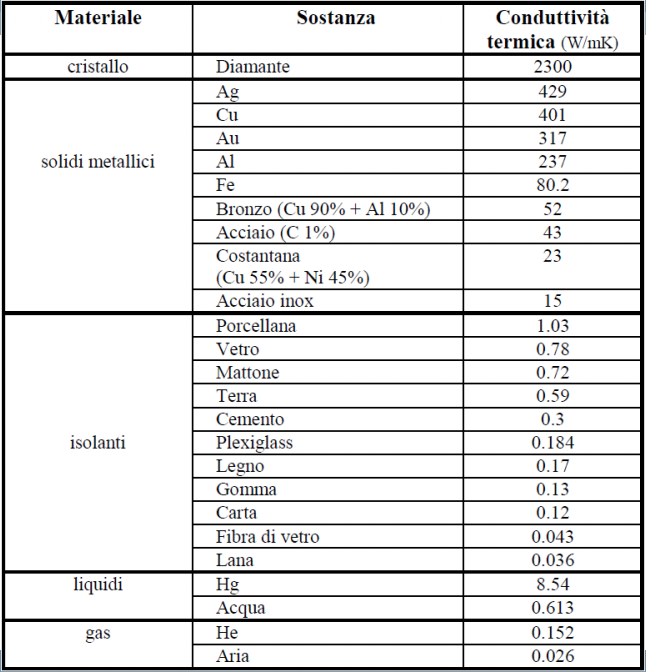
\includegraphics[height=3cm]{../L10/img13.PNG}
\end{center}
\subsection{Coefficiente convettivo}
\textbf{Dipende fortemente} dal tipo di fluido, dalla geometrica e dal tipo di moto (regime, velocità, ecc.).\newline
\newline
\textbf{Valori tipici} per l'acqua e per l'aria sono:
\begin{itemize}
    \item Aria: $h = 5/ 100 [W/m^2K]$;
    \item Acqua: $h = 200/10000 [W/m^2K]$;
    \item Acqua in transizione di fase: $h = 1000/100000 [W/m^2K]$
\end{itemize}